{\chapter{Verstärkendes Lernen}}
\label{sec:rl}
Die meist verbreitetsten und daher auch am bekanntesten Ansätzen im maschinellen Lernen sind das Überwachte Lernen (Supervised Learning) und das Unüberwachte Lernen (Unsupervised Learning). Bei diesen Ansätzen lernt der Algorithmus anhand eines vorliegenden Datensatzes Muster, um diese auf unbekannte Fälle zu übertragen und somit Vorhersagen zu treffen oder Daten zu Gruppieren.

Visualisierung oder Bsp??

Verstärkendes Lernen (Reinforcement Learning) ist ein weiterer Ansatz des maschinellen Lernens bei dem ein Verhalten innerhalb einer festen Umgebung optimiert wird. 

Visualisierung oder Bsp??

Vergleich

\begin{figure}[htb]
  \centering  
  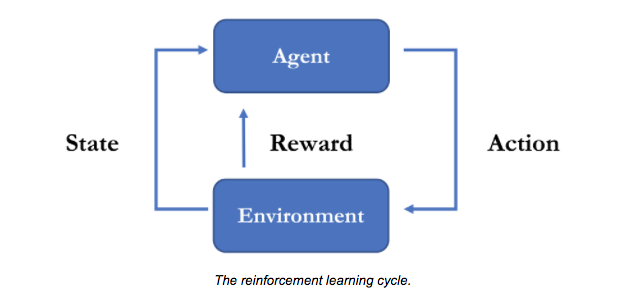
\includegraphics[scale=0.5]{img/rl_cycle.png}
  \caption{Verstärkendes Lernen Ablauf \protect\cite{unity_mlagents_rl_cycle}}
  \label{fig:rl_cycle}
\end{figure}